\section{Introduction}
Un \gls{mid}  est un circuit électronique
dont le support est un substrat thermoplastique moulé par injection, par
opposition aux \glspl{pcb} conventionnels dont le substrat est un composite
plat.

Les \glspl{mid} permettent de regrouper dans une seule pièce des fonctions
mécaniques et éléctroniques. En effet, contrairement aux \glspl{pcb}, les
\glspl{mid} peuvent être conçus en trois dimensions, ce qui réduit
considérablement le nombre de composants et de connecteurs, diminuant ainsi le
temps d'assemblage, et donc le coût du système. 

Les \glspl{mid} ne sont toutefois pas une solution de remplacement des
\glspl{pcb}, car ils ne permettent pas une grande densité de pistes, tandis que
les \glspl{pcb} à plus de deux couches sont désormais peu coûteux et
permettent des circuits à forte densité.


\section{Applications}
Les \glspl{mid} se rencontrent dans des milieux très variés, mais qui ont tous en commun de demander une forte intégration entre l'électronique et la mécanique.

\subsection{Automobile}
L'électronique embarquée dans les voitures devient de plus en plus complexe afin d'augmenter le confort et la sécurité des passagers. 
À l'inverse, le coût d'assemblage, le poids et par conséquent le nombre de pièces doivent être réduits afin de continuer à proposer des modèles abordables.
Les \glspl{mid} sont des solutions adaptées pour remplacer les fils et la connectique, tout en intégrant des fonctions mécaniques, comme des boutons ou de la structure.

À la fig. \ref{fig:mid-automotive-example}, on peut remarquer le gain en simplicité obtenu dans le cas d'un volant multi-fonction.
Ces volants, de plus en plus courants dans les voitures actuelles, permettent au conducteur de changer de chaîne de radio, de rapport de boîte à vitesse, etc.
L'utilisation d'un \gls{mid} a permis ici de simplifier le câblage: Les fils ont été supprimés et les boutons ont été remplacés par des contacts recouvert d'un tapis conducteur en silicone.

\begin{figure}[h]
        \centering
        \begin{subfigure}[t]{0.4\textwidth}
                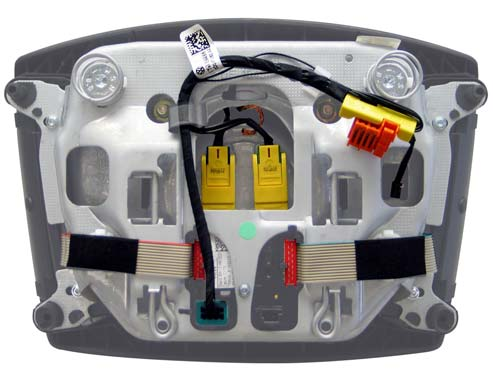
\includegraphics[width=\textwidth]{images/conventional_steering_wheel}
                \caption{Volant multi-fonction conventionnel.}
                \label{fig:conventional-wheel}
        \end{subfigure}%
        ~ 
        \begin{subfigure}[t]{0.4\textwidth}
                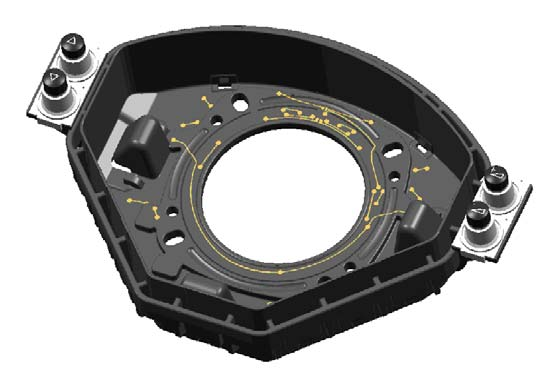
\includegraphics[width=\textwidth]{images/mid_steering_wheel}
                \caption{Volant multi-fonction \gls{mid} (vue \textsc{cao})}
                \label{fig:mid-wheel}
        \end{subfigure}
        \caption{Exemple d'utilisation des \glspl{mid} dans l'automobile.}\label{fig:mid-automotive-example}
\end{figure}

\subsection{Consumer Electronic}
Dans le domaine de l'électronique grand public, la miniaturisation, la diversification et la réduction des coûts posent des difficultés importantes.
Créer une antenne miniaturisée en \textsc{mid} offre deux avantages majeurs par rapport aux antennes classiques et aux \textit{PCB trace antenna} :
\begin{itemize}
    \item L'encombrement est réduit, soit en enroulant l'antenne sur elle même, soit en l'intégrant directement au chassis de l'appareil,
    \item La directivité de l'antenne est parfaitement maîtrisable, permettant ainsi une réception optimale quelque soit l'orientation.
\end{itemize}
La fig. \ref{fig:mid-ce-example} montre l'utilisation des \gls{mid} pour fabriquer une antenne miniature (\SI{4}{\milli\meter} de côté) soudable sur un \gls{pcb} et pour fabriquer une antenne intégrée au chassis d'un smartphone.
Ces images proviennent de la société Molex, qui utilise les \gls{mid} pour la production à très grande échelle et le prototypage de ses antennes.

\begin{figure}[h]
        \centering
        \begin{subfigure}[t]{0.4\textwidth}
                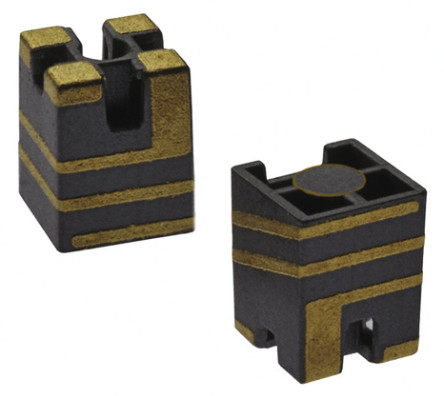
\includegraphics[width=\textwidth]{images/mid-antenna}
                \caption{Antenne soudable sur \gls{pcb}.}
        \end{subfigure}%
        ~ 
        \begin{subfigure}[t]{0.4\textwidth}
                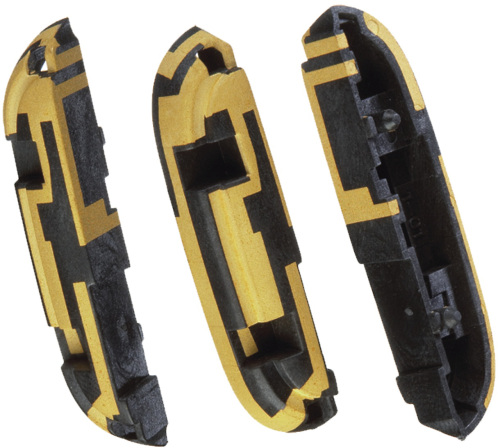
\includegraphics[width=\textwidth]{images/lds-molex-antenna}
                \caption{Antenne intégrée au boîtier.}
        \end{subfigure}
        \caption{Utilisation des \gls{mid} dans les antennes.}\label{fig:mid-ce-example}
\end{figure}

\subsection{Médical}
Une autre application intéressante des \glspl{mid} se situe dans le milieu du médical, et plus particuliérement des implants auditifs.
Ce secteur cherche en effet à miniaturiser de plus en plus ses produits, afin de les rendre plus discrets, ce qui demande une intégration entre électronique et mécanique très poussée.
La fig. \ref{fig:mid-siemens-example} montre l'utilisation faite par Siemens d'un \gls{mid} comme châssis et connecteur d'un implant.
Il n'existe, à notre connaissance, pas d'exemple d'utilisation de \gls{mid} dans des prothèses vitales, comme des stimulateurs cardiaques.


\begin{figure}[h]
    \begin{center}
        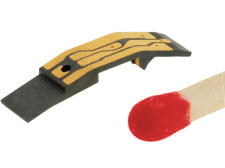
\includegraphics[width=0.3\textwidth]{images/mid-hearing-aid_RED}
        \caption{Chassis d'implant auditif, réalisé en \gls{mid}.}
        \label{fig:mid-siemens-example}
    \end{center}
\end{figure}

